\chapter{绪论}
\section{引言}\label{section 1-1}

随着国民经济和社会的发展,以及人民对美好生活的追求,汽车已成为人们日常生活不可或缺的交通工具之一。
据统计,2021 年底,我国民用汽车保有量高达 30151 万辆 \cite{gou2022zhong}。
然而,汽车数量的急剧增长也给人类社会和自然环境带来了诸多挑战。
据世卫组织数据,全球每年约有 130 万人因道路交通事故死亡,另外约有 2000 至 5000 万人因事故受到如致残等非致命伤害 \cite{shi2022dao}。
同时,日益严峻的城市交通拥堵问题也给经济发展造成了巨大损失。
此外,汽车也是空气污染物排放的主要贡献者之一,仅在 2021 年,全国汽车污染物排放总量就超过 1401.9 万吨 \cite{shen2022zhong}。
近年来,随着传感技术、通讯方式和计算模式的发展,传统汽车正朝着智能化、网联化和协同化方向迅猛发展。
以智能网联汽车(Intelligent Connected Vehicle, ICV)为抓手,车联网(Vehicle-to-Everything, V2X)驱动的智能交通系统(Intelligent Transportation System, ITS)正致力于实现更加安全、高效和可持续发展的下一代交通运输。

近年来,车联网及其推动的智能网联汽车和智能交通系统已上升为我国的重要战略。
2019年9月,国务院发布了《交通强国建设纲要》,提出要加强智能网联汽车的研发,通过新基建形成自主可控的车联网核心技术与生态产业链 \cite{zhong2019jiao}。
2020年2月,国家发改委等11个部委联合发布了《智能汽车创新发展战略》,明确指出发展智能网联汽车对我国的重要战略意义,并将突破关键核心技术作为首要战略任务 \cite{guo2020zi}。
2022年8月,科技部发文支持建设包括智能港口、智能矿山和自动驾驶在内的十个新一代智能示范应用场景\cite{ke2022ke}。
同时,车联网商业化也是业界关注的热点领域。
2019年7月,华为发布了业界首款采用第五代移动通信(The 5th Generation Mobile Communication, 5G)技术的车载通信模组 MH5000,并与一汽、上汽、广汽等 18 家车企共同成立“5G 汽车生态圈”,加速 5G 技术在汽车产业的商业进程,打造智能网联的5G汽车。
2020年10月,超过 100 家相关企业,包括传统汽车制造商、芯片模组与硬件制造商、地图与定位服务提供商在内,于中国上海开展了蜂窝车联网(Cellular-Vehicle-to-Everything, C-V2X)“新四跨”(跨芯片模组、跨终端、跨整车和跨安全平台)应用示范活动。
截至2023年2月,已有十余家车企推出了 C-V2X 量产车型,其中包括一汽、上汽、通用、上汽奥迪、广汽、长安福特、长城、比亚迪和蔚来等。

另一方面,国内外众多一流高校与科研院所围绕车联网、车路协同、无人驾驶、智能交通系统等领域展开了深入探索与研究。
清华大学汽车安全与节能国家重点实验室主任李克强院士团队在提出和推动智能网联汽车“中国方案”技术体系做出了巨大贡献。
中科院复杂系统管理与控制国家重点实验室主任王飞跃院士团队在智能交通的信息物理融合方面取得了重要突破。
无线移动通信国家重点实验室陈山枝教授团队致力于 C-V2X 标准的制定及关键技术的研究,极大推动了车联网产业化进展。
西安电子科技大学综合业务网理论与关键技术国家重点实验室毛国强教授团队在车联网的高效数据分发、实时感知、智能应用等方面均取得了具有国际影响力的科研成果。
深圳大学Victor C.M Leung(梁中明)教授团队专注于车联网边缘缓存、信息安全和无线传输协议等领域的研究,并取得了重要的科研成果。
长安大学赵祥模教授团队在高速公路场景下的智能车路协同体系架构以及相关运行安全性与适应性评估技术方面做出了重要的贡献。

国际上,加拿大滑铁卢大学 Sherman Shen(沈学民)教授团队在车联网安全车路协同、资源优化和智能交通系统等多个领域取得了重要的研究突破。
瑞典奥斯陆大学Yan Zhang(张彦)教授团队在车联网端边云协同、自适应任务协作、负载均衡和隐私保护等方面做出了突出的贡献。
香港理工大学 Jiannong Cao(曹建农)教授团队在车联网边缘计算、大数据与智能交通系统方面取得了重要研究成果。
澳大利亚悉尼大学 Abbas Jamalipour 教授团队在面向下一代网络中车联网通信、感知和计算等方面取得了重要的研究突破。
美国休斯敦大学 Zhu Han(韩竹)教授团队围绕车联网中安全、无线资源分配和管理以及博弈论等方面展开了深入研究并取得了系列重要成果。
加拿大卡尔顿大学 F.Richard Yu(于非)教授团队围绕网联自动驾驶汽车中网络安全和人工智能进行了深入研究,并取得了重要的科研成果。
香港理工大学 Song Guo(郭嵩)教授团队在车联网边缘智能、边缘计算、人工智能等方面做出了突出贡献。
日本东北大学Nei Kato教授团队在车联网中安全、拓扑控制和路由协议等方面进行了全面深入的研究,并获得了系列原创性研究成果。
香港中文大学 Guoliang Xing(刑国良)教授团队在车联网中信息物理融合系统(Cyber-Physical System, CPS)、车路协同、自动驾驶等方面取得了重要研究成果。

“信息物理融合系统”一词是由美国国家科学基金会的Helen Gill约于2006年提出\cite{lee2016introduction}。
自从Li等人\cite{li2011human}于2011年首次将信息物理融合系统应用于车联网中,车载信息物理融合系统(Vehicular Cyber-Physical System, VCPS)\cite{xia2019zi} 已成为国内外学术界热门研究领域之一。
VCPS是一个集智能网联汽车、车联网、边缘计算、云计算等多种技术于一体的系统,利用智能网联汽车的多模态感知能力、V2X 通信技术以及端边云的计算、存储和通信资源,形成一个感知、计算、传输以及控制一体化的综合系统。
然而,由于车联网具有异构高动态、物理环境分布式时变、节点资源动态异构、应用需求多元、真实环境复杂等特点,实现面向异构车联网的车载信息物理融合系统仍然面临巨大挑战。
首先,未来车联网是一个多计算范式、服务架构融合的新型移动网络,融合不同范式并最大化协同效应是实现 VCPS 的基础。
其次,高动态车联网中物理信息动态时变,融合异质感知信息并评估其质量是实现 VCPS 的核心。
再次,车联网中节点资源异构且受限,实现异构资源协同优化以最大化资源利用率是实现 VCPS 的关键。
另外,多元化的 ITS 应用对于车载信息物理融合系统需求具有差异性,实现 VCPS 质量-开销均衡以满足多元应用需求是实现 VCPS 的另一关键。
最后,真实复杂车联网环境中基于 VCPS 的典型应用的部署实现极具挑战且具有重要意义。
因此,本文将结合车联网特点和智能交通系统的多样化应用需求,从服务架构、评估指标、优化策略和原型系统方面进行理论、技术和系统上的综合创新,提炼出异构车联网融合、逻辑视图质量评估、异构资源协同优化、VCPS质量-开销均衡以及复杂真实环境下原型系统实现关键问题,并提出相应的解决方案以实现面向异构车联网的车载信息物理融合系统。

\section{研究背景}\label{section 1-2}

本章节将首先介绍车联网的相关概念及其发展历程,随后以全息路口为例,介绍车载信息物理融合系统,并进一步分析其中所面临的挑战。

\begin{figure}[h]
	\centering
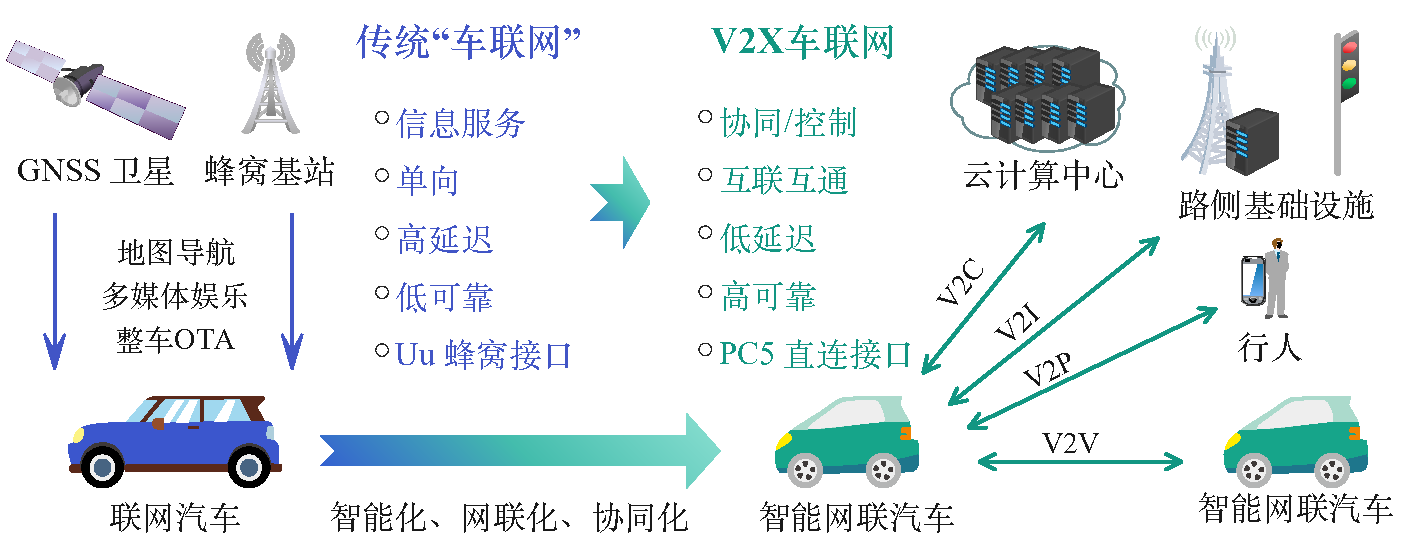
\includegraphics[width=1\columnwidth]{Fig1-1-V2X.pdf}
	\bicaption{从传统“车联网”到V2X车联网}{From traditional `connected vehicles' to V2X communication networks}
	\label{fig 1-1}
\end{figure}

车联网是物联网(Internet of Things, IoT)技术在汽车领域的一种应用形式。
有趣的是,“车联网”概念早在 2G/3G 移动网络时代就已有应用,例如,利用全球导航卫星系统(Global Navigation Satellite System, GNSS)为车辆提供防盗、救援服务。
现今的智能网联汽车(如宝马、比亚迪、福特、通用、蔚来以及特斯拉等诸多汽车厂商产品)大都支持空中下载(Over-the-Air, OTA)技术对其车机系统进行在线更新。
如图 \ref{fig 1-1} 所示,随着汽车朝着智能化、网联化、协同化方向发展,传统面向信息服务的“车联网”也转变为与万物互联互通的 V2X 车联网。
具体而言,V2X 车联网是指多种通讯方式的融合,包括车辆间通讯(Vehicle-to-Vehicle, V2V)、车辆与行人通讯(Vehicle-to-Pedestrian, V2P)、车辆与基础设施通讯(Vehicle-to-Infrastructure, V2I)以及车辆与云端通讯(Vehicle-to-Cloud, V2C)。
车联网利用实时数据分发,实现人、车、路等交通要素的协同配合,最终实现“聪明的车、智慧的路、协同的云”。
进一步,车联网还能配合基于单车智能的自动驾驶技术发展,通过车联网通信协助自动驾驶判断潜在危险,提升道路安全。
随着我国车联网产业在政策规划、标准体系建设、关键技术研发、应用示范和基础设施建设等多方面的稳步发展,车联网的内涵和外延也在不断发展演进\cite{zhong2021che}。
依托快速落地的新型基础设施建设,车联网不仅广泛服务于智能网联汽车的辅助驾驶、自动驾驶等不同应用,并且拓展服务于智慧矿山、智慧港口等企业生产环节以及智慧交通、智慧城市等社会治理领域。

\begin{figure}[h]
	\centering
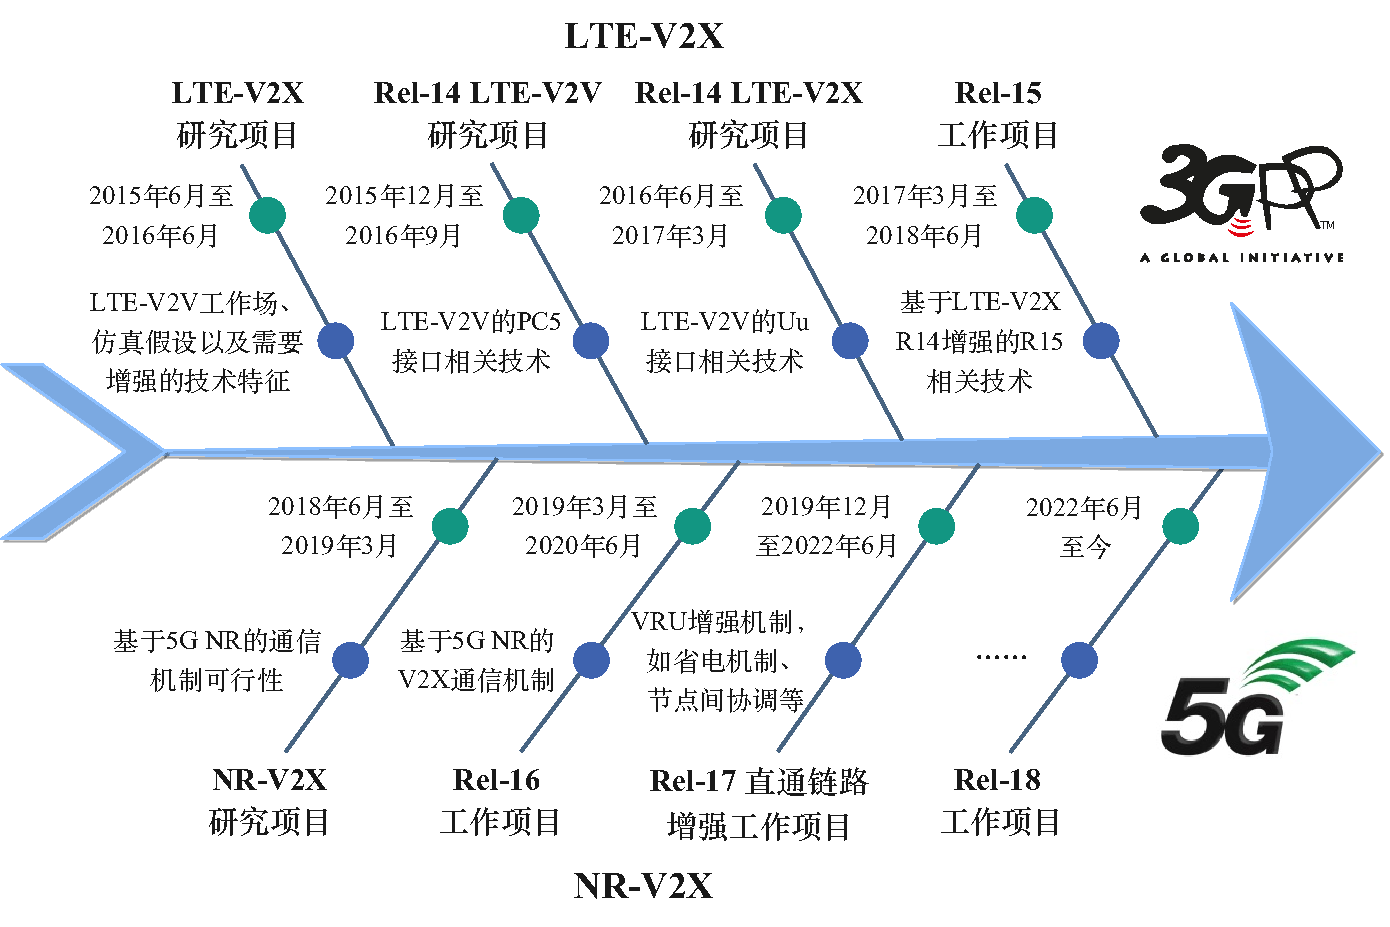
\includegraphics[width=1\columnwidth]{Fig1-2-V2X-evolution.pdf}
	\bicaption{3GPP C-V2X 标准演进}{3GPP C-V2X standard evolution}
	\label{fig 1-2}
\end{figure}

在车联网通信标准方面,电气和电子工程师协会(Institute of Electrical and Electronics Engineers, IEEE)于2003年提出了用于车联网通信的专用短距通信技术(Dedicated Short-Range Communication, DSRC)。
2010年,IEEE正式发布了名为无线接入车载环境(Wireless Access in Vehicular Environments, WAVE)的协议栈,其中包括IEEE 802.11p、IEEE 1609.1/.2/.3/.4协议族和SAE J2735消息集字典 \cite{wu2013vehicular}。
同时,随着基于蜂窝的移动通信技术的快速发展,长期演进(Long-Term Evolution, LTE)的 V2X 通信已经形成了一个较为完善的技术标准体系和产业链 \cite{chen2016lte}。
此外,作为中国 5G 技术创新主要平台的 IMT-2020(5G)推进组于 2017 年成立了 C-V2X 工作组,以加速向基于 5G 的V2X通信演进。
如图 \ref{fig 1-2} 所示,国际标准组织第三代合作伙伴计划(The 3rd Generation Partnership Project, 3GPP)于 2018 年启动基于 5G 新空口(New Radio, NR)的 V2X 标准研究,并于 2020 年完成了Rel-16版本的5G NR-V2X标准\cite{saad2021advancements},且在Rel-17版本中进一步优化了功率控制、资源调度等相关技术。
5G 汽车协会(5G Automotive Association, 5GAA)、下一代移动通信网络(Next Generation Mobile Network, NGMN)联盟以及5G Americas对IEEE 802.11p和C-V2X进行了技术对比,具体结果见表\ref{table 1_1},其表明 C-V2X 在低时延、高可靠性、资源利用率等方面具有技术优势。
目前,我国长期演进车联网通信 LTE-V2X 产业已经蓬勃发展,与 DSRC 的技术路线之争取得了重大进展。
我国已建成基于 LTE-V2X 技术的完备产业链,芯片、模组、车载终端(Onboard Unit, OBU)、路侧设备(Roadside Unit, RSU)等都已成熟且经过了“三跨”“四跨”“新四跨”以及大规模测试,满足了商用部署条件。

\begin{table}[h]\small
\centering
\bicaption[C-V2X和IEEE 802.11p技术对比]{C-V2X和IEEE 802.11p技术对比\cite{cheng2021feng}}[Technical comparisons of C-V2X and IEEE 802.11p]{Technical comparisons of C-V2X and IEEE 802.11p \cite{cheng2021feng}}
\label{table 1_1}
\resizebox{\columnwidth}{!}{%
\begin{tabular}{@{}ccccc@{}}
\toprule
\begin{tabular}[c]{@{}c@{}}C-V2X\\ 技术优势\end{tabular} &
 \begin{tabular}[c]{@{}c@{}}具体技术\\ 或性能\end{tabular} &
IEEE 802.11p &
\begin{tabular}[c]{@{}c@{}}LTE-V2X\\ (3GPP R14/R15)\end{tabular} &
\begin{tabular}[c]{@{}c@{}}NR-V2X\\ (3GPP R16)\end{tabular} \\ \midrule
低时延 &
  时延 &
  不确定时延 &
  \begin{tabular}[c]{@{}c@{}}R14: 20ms\\ R15: 10ms\end{tabular} &
  3ms \\ 
\begin{tabular}[c]{@{}c@{}}低时延/\\ 高可靠\end{tabular} &
  \begin{tabular}[c]{@{}c@{}}资源分配\\ 机制\end{tabular} &
  CSMA/CA &
  \begin{tabular}[c]{@{}c@{}}支持感知+半持续\\ 调度和动态调度\end{tabular} &
  \begin{tabular}[c]{@{}c@{}}支持感知+半持续\\ 调度和动态调度\end{tabular} \\ 
\multirow{3}{*}[3.4ex]{高可靠} &
  可靠性 &
  不保证可靠性 &
  \begin{tabular}[c]{@{}c@{}}R14: \textgreater{}90\%\\ R15: \textgreater{}95\%\end{tabular} &
  支持99.999\% \\  
 &
  信道编码 &
  卷积码 &
  Turbo &
  LDPC \\ 
 &
  重传机制 &
  不支持 &
  \begin{tabular}[c]{@{}c@{}}支持HARQ,\\ 固定2次传输\end{tabular} &
  \begin{tabular}[c]{@{}c@{}}支持HARQ,\\ 传输次数灵活,\\ 最大支持32次传输\end{tabular} \\ 
\multirow{2}{*}[0ex]{\begin{tabular}[c]{@{}c@{}}更远传输\\ 范围\end{tabular}} &
  通信范围 &
  100m &
  \begin{tabular}[c]{@{}c@{}}R14: 320m\\ R15: 500m\end{tabular} &
  1000m \\  
 &
  波形 &
  OFDM &
  \begin{tabular}[c]{@{}c@{}}单载波频分复用\\ (SC-FDM)\end{tabular} &
  循环前缀(CP)-OFDM \\ 
\multirow{2}{*}[1.5ex]{\begin{tabular}[c]{@{}c@{}}更高传输\\ 速率\end{tabular}} &
  \begin{tabular}[c]{@{}c@{}}数据传输\\ 速率\end{tabular} &
  典型6Mbit/s &
  \begin{tabular}[c]{@{}c@{}}R14: 约30Mbit/s\\ R15: 约300Mbit/s\end{tabular} &
  \begin{tabular}[c]{@{}c@{}}与带宽有关,40MHz\\ 时R16单载波2层数据\\ 传输支持约400Mbit/s,\\ 多载波情况下更高\end{tabular} \\ 
 &
  调制方式 &
  64QAM &
  64QAM &
  256QAM \\ \bottomrule
\end{tabular}%
}
\end{table}

\begin{figure}[h] 
	\centering
	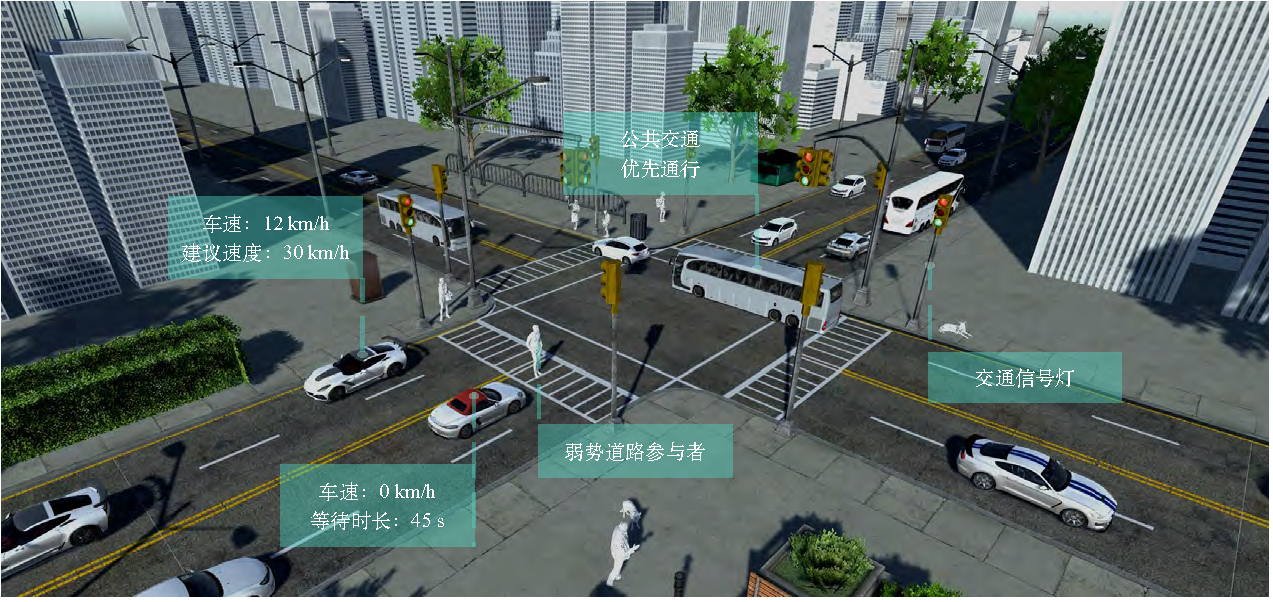
\includegraphics[width=1\columnwidth]{Fig1-3-intersection.pdf}
	\bicaption{基于车载信息物理融合的智慧全息路口应用}{Intelligent holographic intersection application based vehicular cyber-physical systems}
	\label{fig 1-3}
\end{figure}

如图 \ref{fig 1-3} 所示,智慧全息路口是一种基于车载信息物理融合技术的智慧交通管理系统,通过将城市道路上的全要素进行数字化还原,为各类智能交通系统应用提供数据支撑。
智慧全息路口利用道路基础设施和智能网联汽车上搭载的激光雷达、毫米波雷达、摄像头等多源传感设备,对路口进行全方位感知与全要素采集。
这些传感设备可以实时获取交通流量、车速、车道变化等数据,并结合高精度地图呈现路口数字化上帝视角,精准刻画路口上的每一条车道、每一个交通信息灯的状态、每一辆车的行为轨迹等。
在实现路口全要素数字化还原的过程中,全息路口采用了车载边缘计算的技术,将异构感知数据进行融合处理,因而不仅可以提高数据处理速度,还可以降低数据传输成本。
同时,全息路口还利用先进的算法对感知数据进行处理,包括目标检测、目标跟踪、行为分析等,进一步提高数据准确性和精度,从而为后续的交通管理、交通安全和交通规划等应用提供更为可靠的数据基础。

智慧全息路口不仅可以实现路口全要素数字化还原,还可以进一步作为车载信息物理融合系统的外在展示和数据内核,支撑各种智能交通系统的应用,进一步提高城市交通效率和安全性。
例如,全息路口可以为公交优先通行、绿波通行、弱势道路参与者(Vulnerable Road User, VRU)感知等智能交通系统应用提供强有力的支持。
在公交优先通行方面,全息路口可以根据公交车的实时位置和行驶速度,并结合路口的交通状况,提前调整信号控制策略,使公交车获得更好的通行效率和服务。
在绿波通行方面,全息路口可以通过感知路口的交通流量和车速等信息,结合预设的绿波时间和速度,实现路口绿灯时长的自适应调整,从而实现车辆在绿灯通行路段上的无缝衔接和高效通行。
在 VRU 感知方面,全息路口可以利用摄像头等传感设备或V2P通信感知 VRU(如行人、自行车、残疾人等)的存在和行动轨迹,提供实时的路口状态信息和预警信息,保障弱势道路参与者的交通安全和通行便利。

通过以上讨论可知,实现车载信息物理融合系统是实现各类智能交通系统应用的基础。
然而,在高异构、高动态、分布式、资源受限的车联网中实现车载信息物理融合系统以满足多元 ITS 应用需求仍然面临着诸多问题和挑战。
因此,针对这些问题和挑战,需要进一步展开深入全面的研究。
具体来说,首先,异构车联网亟需融合创新。
未来车联网是一个多服务范式并存的高异构移动网络,因此需要研究异构车联网融合服务架构,最大化不同服务范式的协同效应,以支持 VCPS 的部署实现。
此外,为了提高 VCPS 的实时性和可靠性,还需要针对异构车联网的实时通信特点,开发高效的跨层通信协议和传输机制。
其次,车载信息物理融合系统评估指标亟需设计。现有研究都缺乏针对基于多源异质感知信息融合的 VCPS 进行整体深入的评估。
因此,需要研究 VCPS 质量评估指标,并通过控制车辆感知行为与资源分配进一步提升 VCPS 系统质量。
再次,异构资源亟需协同优化。
车联网中的通信和计算资源分布在不同的车辆和基础设施中,因此需要针对异构资源进行协同优化,以提高系统的整体性能和效率。
另外,车载信息物理融合系统亟需质量-开销均衡优化。
在车联网中,车载信息物理融合系统需要保证实时性和准确性的同时,还需要考虑资源开销和能耗问题。
因此,需要研究质量-开销均衡的优化策略,以提高系统的资源利用率和能耗效率。
最后,亟需实现车载信息物理融合系统的原型以验证其性能。
通过仿真模拟实验测试和真实车联网环境中原型系统搭建,可以进一步验证车载信息物理融合系统的可行性和有效性,为其在实际应用中提供更为可靠的支持和保障。
本文将从以上几个方面针对面向异构车联网的车载信息物理融合系统的国内外研究现状展开深入全面的讨论。

\section{国内外研究现状}\label{section 1-3}

面向异构车联网的车载信息物理融合系统是实现各类智能交通系统应用的基础,其已成为国内外学术界的研究热点之一。
本章节对国内外相关研究工作进行了梳理和总结,现从以下几个方面进行详细阐述。

\subsection{车联网服务架构研究与现状}

随着智能交通系统应用的不断涌现,传统的基于静态的网络拓扑和硬件设备的车联网架构已无法适应大规模、高可靠、低时延的智能交通系统应用需求。
因此,研究人员正致力于将软件定义网络(Software Defined Network, SDN)新范式应用于车联网中,其通过数据平面和控制平面的分离,实现了高度灵活的数据调度策略和网络功能虚拟化。
Liu等人 \cite{liu2016cooperative} 提出了在软件定义车联网(Software Defined Vehicular Network, SDVN)中基于混合 I2V/V2V 通信的在线协同数据调度算法以提高数据分发的性能,其为 SDN 概念在车联网中的首次实现。
Dai等人\cite{dai2018cooperative}提出了在基于SDN的异构车联网中具有时间约束的时态信息服务的调度。
Luo等人\cite{luo2018sdnmac}提出了一个基于SDN的媒体接入(Media Access Control, MAC)协议,以提高动态车联网环境中的通信性能。
Liu等人\cite{liu2018coding}提出了一个基于SDN的服务架构,并结合车辆缓存和网络编码来提高带宽效率。
Zhang等人\cite{zhang2022ac-sdvn}提出了一种解决 SDVN 中视频组播安全问题的安全访问控制协议,实现了多播视频请求车辆和RSU的身份认证。
Zhao等人\cite{zhao2022elite}提出了一种基于智能数字孪生技术的软件定义车联网的分层路由方案,克服了 SDVN 架构中高动态拓扑局限性。
Lin等人\cite{lin2023alps}提出了一种适用于 SDVN 的自适应链路状态感知方案,能够在信标间隔内及时获取链路状态信息,减少数据包丢失。
Ahmed等人\cite{ahmed2023deep}提出了一个用于 SDVN 中车辆传感器负载均衡的算法,并提出了一个数据包级入侵检测模型,可以跟踪并有效识别网络攻击。
然而,现有大部分工作都仅是在软件定义车联网架构的基础上从数据分发、路由缓存、数据安全等方面展开了研究,缺乏对整体架构的深入分析。

移动边缘计算(Mobile Edge Computing, MEC)\cite{mao2017a}作为应用于移动网络的新范式,通过将计算、存储和网络资源靠近移动终端设备,MEC可以提供更快速、更可靠的服务,同时减少网络流量和延迟。
越来越多的研究在车联网环境中考虑将移动边缘计算范式以提高系统实时性、可靠性、安全性。
Liu等人\cite{liu2017a}首次将移动边缘计算范式融入车联网,并集成了不同类型的接入技术,以提供低延迟和高可靠性的通信。
Lang等人\cite{lang2022cooperative}提出了一种基于区块链技术的车载边缘计算(Vehicular Edge Computing, VEC)中的合作计算卸载方案,以提高网络资源的利用效率,并确保计算卸载的安全性。
Liu等人\cite{liu2021fog}研究了端边云协同架构中的合作数据传播问题,并提出了一种基于Clique的算法来联合调度网络编码和数据分发。
Dai等人\cite{dai2021edge}设计了一个基于自适应比特率的多媒体流的VEC架构,其中边缘缓存和传输服务被提供给以不同质量等级编码的文件块。
Zhang等人\cite{zhang2022digital}提出了一种车载边缘缓存技术,其基于用户偏好的相似性和服务的可用性,动态地协调边缘节点和车辆的缓存能力。
Liu等人\cite{liu2020adaptive}提出了一个两层的VEC架构,利用云、静态边缘节点和移动边缘节点来处理时延敏感性任务。
Liao等人\cite{liao2021learning}提出了一种空地一体的VEC任务卸载策略,其中车辆能够学习具有多维意图的长期策略。
Liu等人\cite{liu2023mobility}提出了一种车辆计算任务卸载方案,通过对车辆的移动性分析,利用车辆计算资源来提高VEC场景下任务执行的效率和用户体验。
Liu等人\cite{liu2023asynchronous}提出了一种分布式VEC任务卸载和资源管理的联合优化问题,并采用异步深度强化学习算法来寻找最优解。
然而,上述研究并没有综合考虑异构车联网中最大化不同服务架构的协同效应,且绝大多数架构研究仍停留在理论分析层面,缺乏在实际场景中对架构优势进行验证。

\subsection{车载信息物理融合系统评估指标研究与现状}

随着车载信息物理融合系统的发展,越来越多的研究人员聚焦于VCPS 中的预测、调度和控制技术,旨在有效提高VCPS系统的整体性能和可靠性。
在预测技术方面,Zhang等人\cite{zhang2021a}提出了一种基于VCPS架构的车辆速度曲线预测方法,其通过协同使用VCPS中的不同控制单元来完成速度曲线预测。
Zhang等人\cite{zhang2019a}提出了一种混合车辆速度预测方法,该方法将交通流状态与个人驾驶行为相结合。
Albaba等人\cite{albaba2021driver}将深度Q网络(Deep Q Networks, DQN)和层次博弈论结合起来,对高速公路驾驶场景中的司机进行行为预测,其中k级推理被用来模拟人类司机的决策过程。
Zhang等人\cite{zhang2020data}在变道行为预测模型和加速预测模型的基础上预测了车辆状态,并通过动态路由算法,实现车辆之间的协同合作,以优化资源利用率和降低能源消耗。
Zhou等人\cite{zhou2021wide}提出了一种基于宽-注意力和深度-组合模型用于交通流量预测,其中,宽-注意力模块通过自注意机制线性模型从交通流中提取全局关键特征,深度-组合模块则通过卷积神经网络和长短时记忆网络组件来推广局部关键特征。
在调度技术方面,Li等人\cite{li2020cyber}考虑了车辆的流动性,并开发了一个基于物理比率-K干扰模型的广播方案以确保通信的可靠性。
Lian等人\cite{lian2021cyber}提出了一种基于既定地图模型的路径规划的调度方法,以优化路径利用效率。
在控制技术方面,Dai等人\cite{dai2016a}提出了一种自主交叉口控制机制,以确定车辆通过交叉口的优先权。
Hu等人\cite{hu2017cyber}提出了一种燃油最优控制器,根据领先车辆的状态优化车辆速度和无级变速箱齿轮比。
Lv等人\cite{lv2018driving}提出了一种自适应算法,用于控制三种典型驾驶方式下不同协议选择的车辆加速。
这些研究集中在支持VCPS的不同技术上,如轨迹预测、路径调度和车辆控制,这促进了各种ITS应用的实施。
然而,这些研究是基于对车联网中物理元素建模的高质量信息可用性的假设,并没有对车载信息物理融合系统的质量进行定量分析。

部分研究工作侧重于利用深度强化学习(Deep Reinforcement Learning, DRL)优化 VCPS 中车辆感知和信息融合。
Dong等人\cite{dong2020spatio}提出了一种基于 DQN 的方法,以融合在本地环境中获得的信息,从而做出可靠的车道变更决策。
Zhao等人\cite{zhao2020social}设计了一个基于近似策略优化的社会意识激励机制,以得出最佳的长期车辆感知策略。
Mika等人\cite{mlika2022deep}提出了一个基于深度确定性策略梯度(Deep Deterministic Policy Gradient, DDPG)的解决方案,通过调度资源块和广播覆盖来优化信息时效性。
然而,上述算法不能直接应用于VCPS中的协同感知和异构信息融合,而且当考虑到多辆车场景时,上述算法并不适用。
另一方面,已有部分研究对VCPS中的信息质量进行了评估。
Liu等人\cite{liu2014temporal}提出了一种用于VCPS中时态数据传播的调度算法,其在实时数据传播和及时信息感知之间取得了平衡。
Dai等人\cite{dai2019temporal}提出了一种进化的多目标算法,以提高信息质量与改善数据到达率。
Liu等人\cite{liu2014scheduling}提出了两种在线算法,通过分析传播特性来调度不同一致性要求下的时态数据传播。
Rager等人\cite{rager2017scalability}开发了一个框架,通过对随机数据负载进行建模来提高信息质量,以捕捉真实网络的随机性。
Yoon等人\cite{yoon2021performance}提出了一个统一的合作感知框架,考虑到车联网中的通信损耗和车辆的随机运动,以获得车辆的精确运动状态。
上述研究主要集中在VCPS中数据及时性、准确性或一致性方面的信息质量评估。
然而,上述研究仅考虑了同质数据项层面的质量评估,这在考虑应用层面时是不充分的。

\subsection{车联网资源分配与任务卸载研究与现状}

车联网中的资源分配一直是学术界的研究热点 \cite{noor-a-rahim2022a},大量研究人员针对车联网中通信资源分配进行了深入研究。
He等人\cite{he2022meta}提出了一种针对动态车联网环境的资源管理框架,其采用马尔科夫决策过程和分层强化学习相结合的方法,可以快速适应不同场景,并显著提高动态车联网的资源管理性能。
Lu等人\cite{lu2021user}提出了一种基于用户行为的虚拟网络资源管理方法,集成学习预测用户的语音通话持续时间和流量使用情况,以进一步优化现有的车联网通信。
Peng等人\cite{peng2020deep}提出了一种针对车联网的资源管理方案,通过应用DDPG方法解决了多维资源优化问题,实现了资源快速分配和满足车联网服务质量(Quality of Service, QoS)要求。
Wei等人\cite{wei2022multi}针对车联网云计算中的资源分配问题,从提供者和用户双重视角进行了优化,提出了一种改进的NSGA-II算法来实现多目标优化。
Peng等人\cite{peng2021multi}研究了在无人机辅助车联网中进行多维资源管理的问题,提出了一种基于多智能体深度确定性策略梯度(Multi-Agent Deep Deterministic Policy Gradient, MADDPG)的分布式优化方法,实现了车辆的联合资源分配和QoS要求的满足。
为了进一步提高频谱利用率和支持更多车辆接入,部分研究人员已经将非正交多址接入(Non-Orthogonal Multiple Access, NOMA)技术融入于车联网中。
Patel等人\cite{patel2021performance}评估了基于NOMA的车联网的通信容量,数值结果显示,NOMA通信容量比传统的正交多址接入高出约20\%。
Zhang等人\cite{zhang2021centralized}利用基于图的匹配方法和非合作博弈分布式功率控制,为NOMA车联网开发了一个集中的两阶段资源分配策略。
Zhu等人\cite{zhu2021decentralized}提出了一种考虑随机任务到达和信道波动的最优功率分配策略,以最大化长期的功率消耗和延迟。
Liu等人\cite{liu2019energy}提出了在基于NOMA的车联网中功率分配的交替方向乘子法算法。
尽管如此,这些研究主要是基于单边缘节点的情况,无法处理不同边缘节点之间的相互干扰情况。

随着车载边缘计算的发展,越来越多研究专注于VEC中的任务卸载或资源分配。
Liu等人\cite{liu2021rtds}通过评估VEC中的移动性感知的通信模型、资源感知的计算模型和截止时间感知的奖励模型,提出了一种多周期任务卸载的实时分布式方法。
Shang等人\cite{shang2021deep}研究了节能的任务卸载,并开发了一种基于深度学习的算法来最小化能耗。
Liu等人\cite{liu2022a}提出了一种结合交替方向乘子法和粒子群优化的任务卸载算法,以最小化执行延迟、能源消耗和支付成本的加权和。
Chen等人\cite{chen2020robust}提出了一种带有故障恢复功能的计算卸载方法,以减少能源使用并缩短应用完成时间。
Pan等人\cite{pan2022asynchronous}提出了一种基于异步联合深度强化学习算法的计算卸载方案,旨在实现在车联网中的超高可靠低时延通信(ultra-Reliable and Low-Latency Communication, uRLLC)服务需求下的吞吐量最大化。
Zhu等人\cite{zhu2022a}提出了一种用于智能反射面辅助下的VEC的动态任务调度算法,考虑了车辆的移动模式、传输条件和任务大小以及并发传输之间的相互干扰,并优化了有限的处理器和资源的分配。
另外,部分研究聚焦于在车联网中使用多智能体强化学习(Multi-Agent Deep Reinforcement Learning, MADRL)\cite{althamary2019a}的任务卸载或资源分配。
Alam等人\cite{alam2022multi}开发了一种基于深度强化学习的多代理匈牙利算法,用于VEC中的动态任务卸载,以保证延迟、能耗和支付费用的要求。
Zhang等人\cite{zhang2021adaptive}提出了一种用于边缘资源分配的MADDPG方法,以在严格的延迟约束下最小化车辆任务卸载成本。
He等人\cite{he2021efficient}提出了一种多代理行动者-评论家(Multi-Agent Actor-Critic, MAAC)算法,为具有严格延迟要求和最小带宽消耗的车辆分配资源。
尽管如此,这些解决方案只考虑了车联网中单一类型的智能体(即车辆或边缘节点)。
同时,以上研究工作都没有研究实时任务卸载和通信/计算资源分配的协同效应。

部分研究考虑了VEC的联合通信和计算资源分配。
Cui等人\cite{cui2021reinforcement}提出了一种多目标的强化学习方法,通过结合通信和计算资源分配来减少系统延迟。
Han等人\cite{han2020reliability}通过动态编程方法提出了面向耦合的车辆通信和计算的可靠性计算。
Xu等人\cite{xu2021socially}采用契约理论为每个潜在的内容供应商和内容请求者对分配通信和计算资源。
少数研究者研究了联合任务卸载和资源分配。
Dai等人\cite{dai2021asynchronous}提出了一个异步的深度强化学习,用于考虑异构服务器的数据驱动的任务卸载,如车辆、VEC服务器和云。
Dai等人 \cite{dai2022a}开发了一种概率计算卸载方法,用于根据边缘节点的计算分配概率独立调度计算卸载。
Nie等人\cite{nie2021semi}提出了一种多智能体联合强化学习算法,在无人机支持的VEC中联合优化资源分配和功率控制。
然而,现有研究主要是基于集中式调度,具有较高的通信开销和调度复杂性,不适用于大规模的车联网。

\subsection{车载信息物理融合中质量/开销优化研究与现状}

大量研究人员针对车载信息物理融合中服务质量优化问题进行了深入研究,致力于提高智能交通系统应用的用户体验和网络效率。
Wang等人\cite{wang2016offloading}提出了一种组合优化的方法,以减少移动数据流量以满足 VCPS 中面向服务质量的服务需求。
Jindal等人\cite{jindal2018sedative}提出了一种基于 SDN 和深度学习的VCPS网络流量控制方案,其有效地解决VCPS中的网络流量管理问题,为VCPS提供更好的服务质量。
Zhu等人\cite{zhu2022joint}提出了一种基于双时间尺度深度强化学习的方法,用于优化基于编队的 VCPS 中的车辆间距和通信效率,同时满足V2I通信的服务质量要求。
Wang等人\cite{wang2023a}提出了一种基于公交车聚类和混合数据调度的集群式车辆间通信方法,用于在城市场景下实现车联网混合数据传播,实现了从公交车到普通车辆的有效数据传播并满足了严格和个性化的QoS需求。
Chen等人\cite{chen2021qos}研究了可重构智能表面辅助车联网中的频谱共享问题,旨在通过优化车辆的发送功率、多用户检测矩阵、车辆间频谱重用以及智能表面反射系数等参数,提高车联网通信的服务质量。
Lai等人\cite{lai2017a}提出了一种基于 SDN 的缓存感知流媒体传输方法,其根据用户的移动信息、播放缓冲区的状态和当前网络信号的强度,向SDN控制器提供流媒体传输策略,以实现最小延迟和更好的服务质量。
Tian等人\cite{tian2022multiagent}提出了一种基于 MADRL 的资源分配框架,以共同优化信道分配和功率控制,满足车联网中的异构服务质量需求。
Zhang等人\cite{zhang2020hierarchical}研究了 MEC 车联网中,联合分配频谱、计算和存储资源的问题,并利用深度确定性策略梯度解决该问题,以满足车联网应用的服务质量要求。
Sodhro等人\cite{sodhro2020ai}提出了一个可靠、无干扰的移动管理算法,解决了车内网络中的通信、计算和存储空间等方面的问题,并提出了可靠和延迟容忍的无线信道模型和多层边缘计算驱动的车间框架,显著提升了车联网服务质量。

另一方面,部分研究人员致力于降低 VCPS 中的各类开销。
Zhao等人\cite{zhao2021a}提出了一种基于 SDN 和无人机辅助的车辆计算卸载优化框架,设计了UAV辅助车辆计算成本优化算法,以最小化车辆计算任务的系统成本。
Zhang等人\cite{zhang2019hybrid}提出了一种基于蚁群优化和三个变异算子的算法优化具有灵活时间窗口的多目标车辆路径,旨在最小化行驶成本和固定车辆成本。
Ning等人\cite{ning2020when}针对 5G 车联网中的有限无线频谱和能源供应问题,构建了一个智能卸载框架,通过联合利用蜂窝频谱和未许可频谱来满足车辆需求并在考虑时延限制基础上使成本最小化。
Tan等人\cite{tan2019twin}提出了一种基于人工智能的多时间尺度框架的联合通信、缓存和计算策略,其考虑车辆的移动性和硬服务截止期限约束,并实现最大化车载网络的成本效益。
Hui等人\cite{hui2022collaboration}提出了一种基于数字孪生技术的协作自动驾驶方案,并通过联盟博弈机制来确定最佳车辆分 组,以最小化每个组的计算成本和传输成本。
进一步,部分研究人员考虑 VCPS 中不同目标的均衡问题。
Heo等人\cite{heo2019performance}提出了使用巴士作为移动 RSU 的性能和成本权衡研究,以解决静态 RSU 高昂的部署和管理成本问题。
Yadav等人\cite{yadav2020energy}提出了一种节能动态计算卸载和资源分配方案,解决了车联网中存在的能量-延迟权衡和有效的资源分配机制等问题。
Zhang等人\cite{zhang2022low}研究了信息为中心的车联网的内容服务,提出了以路侧设备为中心和请求自适应两种缓存更新和内容传递方案,以平衡信息新鲜度和服务延迟。
然而,上述研究均未考虑车载信息物理融合系统构建的质量和开销,缺乏对于 VCPS 系统本身评估与质量-开销均衡的深入分析。

\subsection{智能交通系统安全相关应用研究与现状}

随着城市化进程的加速和交通流量的不断增加,智能交通系统安全相关应用的部署可以大幅提高道路交通的安全性,减少交通事故的发生,保障公众的生命财产安全。
大量研究人员针对驾驶员状态监测、驾驶行为分析、交通监测等方面展开了研究。
Mugabarigira等人\cite{mugabarigira2023context}提出了一种基于车辆行为追踪和驾驶风险分析的导航系统,可以提高城市道路上驾驶车辆的安全性。
Chang等人\cite{chang2018design}提出了一种基于可穿戴智能眼镜的疲劳驾驶检测系统,可以实时检测车辆驾驶员的疲劳或嗜睡状态。
Dutta等人\cite{dutta2022design}提出了一种基于凸优化的鲁棒分布式状态估计系统,用于保护连接车辆的传感器数据免受拒绝服务或虚假数据注入攻击。
Wang等人\cite{wang2021deep}提出了一种使用深度学习加速器的嵌入式平台上鲁棒的雨滴检测系统,并利用该检测结果自动控制汽车雨刷。
Sun等人\cite{sun2022toward}提出了一种有效的交通估计系统,可以通过与过往车辆的通信并记录其出现情况来实现自动交通测量,从而为智能交通系统提供关键信息。

部分研究工作从车辆控制、车辆编队控制、路口交通流控制等多个层面对ITS安全相关应用展开了深入分析。
Zhang等人\cite{zhang2021data}提出了一种面向智能交通的分布式安全巡航控制系统,利用历史数据建立了车辆行为预测模型和动态驾驶系统模型,并设计了考虑合并行为概率的安全跟驰控制策略。
Zhao等人\cite{zhao2022resilient}提出了一个具有鲁棒性的车辆编队控制系统,并设计了一种在多重干扰和拒绝服务攻击下恢复机制,限制拒绝服务攻击对VCPS的不利影响的时间持续率和发生频率。
Zhu等人\cite{zhu2022joint}针对基于编队的VCPS中车辆间距离和V2I通信效率的权衡问题,提出了编队的波束成形和间距控制系统,其中设计了一个基于软行动者-评论家算法的双时间尺度深度强化学习算法来学习有效的控制策略。
Pan等人\cite{pan2023privacy}提出了一种面向车联网的车队隐私保护集结控制系统,其中提出了一种基于分布式比例积分观察器的状态估计方法,并通过采样数据的动态加密和解密方案,使得车队之间的通信数据得以保密。
Li等人\cite{li2021confidenitality}介绍了一种全面的低延迟协作安全车辆编队数据传播系统,其采用一种基于车队之间的无线电信道相关性的协作密钥协商协议。
Kamal等人\cite{kamal2021control}提出了一种多智能体路口交通流控制系统,其中使用名为广播控制多智能体系统的随机梯度方法来计算即将到来的交通信号灯持续时间。
Lian等人\cite{lian2021cyber}提出了基于交通控制方法的智能物流系统,其中基于路径网络模型的特点,实现了改进的A*路径规划算法,以实现时间的敏感性主动调度和碰撞避免。

车辆碰撞预警系统通过实时监测车辆周围的交通情况,能够及时发现和预警潜在的碰撞危险,减少交通事故的发生。
其作为一种典型车辆主动式安全应用,已吸引广大研究人员的注意。
现有的大多数车辆碰撞预警系统都是基于超声波雷达或激光雷达等测距传感器的。
Song等人\cite{song2018real}提出了一种用于车辆主动安全系统中的实时障碍物检测和状态分类方法,采用立体摄像头和毫米波雷达进行融合,结合车辆运动模型,通过多个模块感知环境,准确快速地判断出“潜在危险”物体。
Wu等人\cite{wu2019series}提出了一种77GHz车辆碰撞预警雷达系统短程天线,该系统采用补丁阵列天线作为基本结构,并采用多层板设计技术使其尺寸更小。
然而,这些方案都存在非视距(Non-Line-Of-Sight, NLOS)的问题,即在障碍物遮挡情况下基于视距(Line-Of-Sight, LOS)的方法不再适用。
近年来,随着计算机视觉的发展,一些研究集中在基于摄像头实时视频流的碰撞检测上。
Wang等人\cite{wang2016vision}提出了一种新颖的车辆制动行为检测方法,利用安装在测试车挡风玻璃上的彩色摄像头或移动设备来捕获前车信息,以避免车辆与前方车辆相撞。
Song等人\cite{song2018lane}提出了一种轻量级的基于立体视觉的行车道检测和分类系统,以实现车辆的横向定位和前向碰撞警告。
然而,基于计算机视觉的方法可能需要密集的计算和大量的数据传输,这使得系统的性能无法得到实时响应。 
另一方面,一些研究考虑了通过V2X通信进行碰撞预警。
Hafner等人\cite{hafner2013cooperative}利用V2V通信技术实现了计算效率高的分布式算法,用于交叉路口的车辆协同防撞,并对所提方法进行了实验验证。
Gelbar等人\cite{gelbal2017elastic}提出了一个基于V2X通信的车辆碰撞预警和避免系统,并使用硬件在环模拟证明了所提方法的有效性。
然而,无线通信中传输时延和数据包丢失等内在特征是不可避免的,而且对于车辆碰撞预警系统来说也是不可忽视的,这使得在真实复杂车联网环境中实现实时和可靠的安全关键型服务变得更加困难。

\section{研究目标与研究内容}\label{section 1-4}
\subsection{研究目标}

本文针对高动态异构车联网融合、分布式时变车联网物理环境、动态异构车联网节点资源、多元智能交通系统应用需求,以及真实复杂车联网环境所带来的挑战,从服务架构融合、评估指标设计、协同资源优化、质量-开销均衡以及原型系统实现五个方面对面向异构车联网的车载信息物理融合系统展开研究。
基于上述描述,本文的研究目标包括如下:

\circled{1} 实现面向异构车联网的融合服务架构,为车载信息物理融合系统提供架构基础。首先,结合软件定义网络、网络功能虚拟化(Network Functions Virtualization, NFV)与网络切片等关键思想,提出基于 SDN 的分层服务架构,以支持系统面向大规模数据服务的灵活性、可靠性及可扩展性。其次,考虑控制层、虚拟化层、数据层面临的挑战,设计跨层协议栈。最后,基于边缘计算范式的分布式服务,实现集中控制与分布式调度的有机结合,进一步提高系统的可靠性与可扩展性。

\circled{2} 实现面向车联网时变物理信息的分布式感知与异质信息融合,为车载信息物理融合系统提供数据支撑。首先,面向车载边缘计算环境,提出基于多类M/G/1优先队列的感知信息排队模型。进一步,针对边缘视图对于感知信息的时效性、完整性以及一致性需求,设计VCPS评估指标,实现车辆协同信息感知与边缘侧的异质信息融合。最后,建立边缘视图质量评估模型,并基于多智能体强化学习,提出针对边缘视图质量的物理感知优化策略,实现高效实时的边缘视图构建。

\circled{3} 实现面向动态车联网节点的异构资源协同优化,为车载信息物理融合系统提供技术支持。首先,面向NOMA车联网的车载边缘计算环境,提出 V2I 传输与任务卸载模型。进一步,建立协同资源优化博弈模型,并将其分解为资源调度与任务卸载两个子问题。最后,针对资源调度子问题,基于凸优化理论提出最优资源分配策略;针对任务卸载子问题,基于多智能体 D4PG 算法提出任务卸载策略,实现基于边缘协同的异构资源优化。

\circled{4} 实现面向多元智能交通系统应用需求的 VCPS 质量-开销均衡优化,为车载信息物理融合系统提供理论保障。首先,面向多元智能交通系统应用需求,针对车联网中不同交通要素,建立相应的数字孪生模型。进一步,综合考虑数字孪生模型的差异性数据需求,建立车载信息物理融合系统的质量与开销模型。最后,基于多目标强化学习,提出车载信息物理融合系统的质量与开销均衡策略,实现质量-开销均衡的车载信息物理融合。

\circled{5} 建立软件仿真环境、硬件在环测试平台,以及基于无人小车的验证平台,综合验证所提模型、机制与算法的可行性与有效性。首先,基于真实车辆轨迹与地图信息搭建交通仿真平台。其次,搭建基于真实OBU(端)、RSU(边)的通信与计算环境,及基于LTE/5G 的远程服务器通信与计算平台(云),实现硬件在环性能验证。最后,基于真实车联网环境,实现基于车载信息物理融合的超视距碰撞预警原型系统,进一步验证所提算法与系统模型。

\subsection{研究内容}

本文致力于研究面向异构车联网的车载信息物理融合系统,主要研究内容及关系如图 \ref{fig 1-4} 所示。
首先,面向高动态异构车联网,融合不同的计算范式与服务架构是实现车载信息物理融合的基础。
因此,本文将首先研究如何设计基于软件定义网络和边缘计算的融合车联网架构。
其次,面向分布式时变物理环境,有效的数据获取与建模评估是驱动车载信息物理融合的核心。
因此,本文将研究如何评估并提高车载边缘侧所构建的逻辑视图质量。
再次,面对动态异构节点资源,高效的任务调度与资源分配是进一步提升智能交通系统服务质量的关键。
因此,本文将进一步研究如何实现异构资源协同优化,提高异构资源利用效率。
面向多元智能交通系统应用需求,满足差异性的系统质量与系统开销是驱动车载信息物理融合的另一关键。
因此,本文将更进一步研究VCPS质量/开销模型及其优化策略。
最后,面向真实复杂车联网环境,基于车载信息物理融合系统进行有效设计并实现具体系统原型是具有挑战的。
因此,本文将深入研究基于车载信息物理融合的超视距碰撞预警原型系统设计与实现。
本文具体研究内容如下所述。

\begin{figure}[h] 
	\centering
	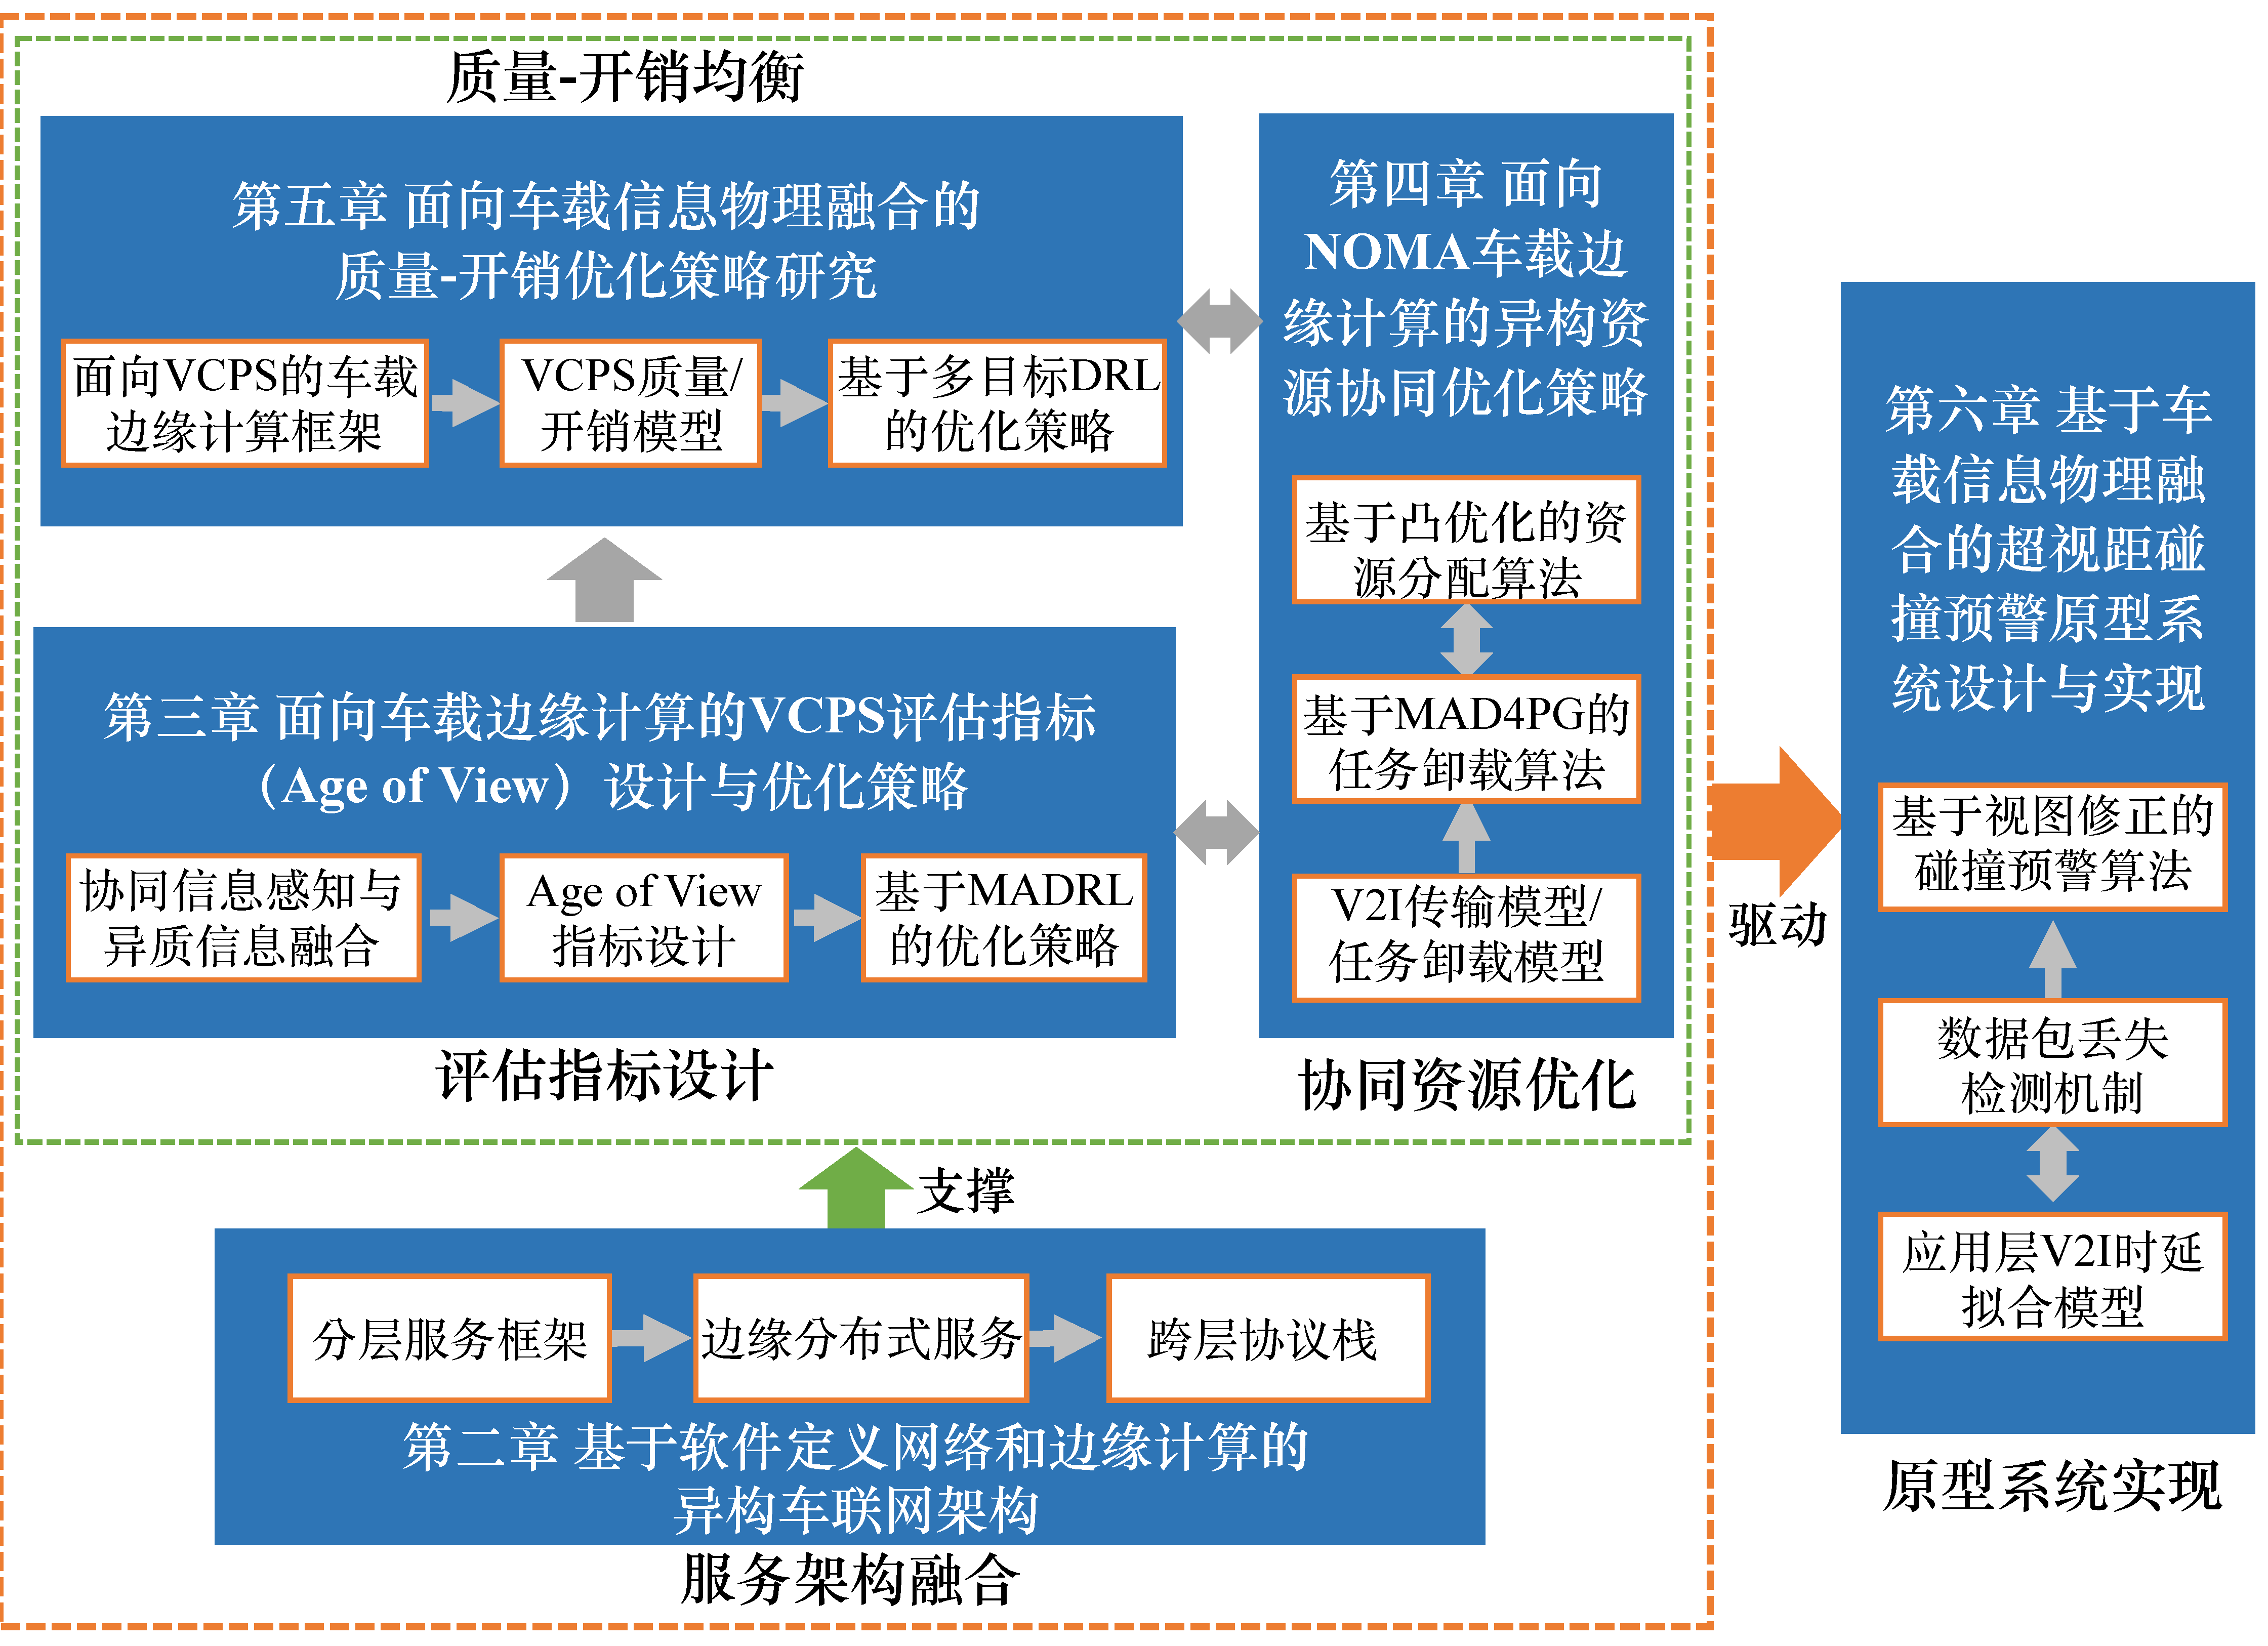
\includegraphics[width=1\columnwidth]{Fig1-4-content.pdf}
	\bicaption{主要研究内容}{Main research content}
	\label{fig 1-4}
\end{figure}

\circled{1} 基于软件定义网络和边缘计算的异构车联网架构研究。
考虑车联网环境中的网络资源的高异构性、拓扑结构的高动态性,以及车辆节点的高移动性等关键特征,本文将以软件定义网络为基础,结合网络功能虚拟化、边缘计算与网络切片等关键思想,提出基于 SDN 和边缘计算的异构融合车联网架构。本部分将重点研究基于 SDN 的异构网络分层服务架构、基于边缘计算的网络融合与分布式控制策略以及跨层协议栈。

\circled{2} 面向车载边缘计算的 VCPS 评估指标(Age of View)设计与优化策略研究。
考虑车联网物理环境分布式时变性、感知信息维度与来源不同,以及车辆节点感知能力差异等关键特征,本文将针对物理信息的感知与建模进行研究,并提出车载信息物理融合系统评估指标与优化策略。本部分将重点研究车载边缘计算环境下车辆协同感知与边缘侧异质信息融合模型,进一步考虑信息的多维需求(时效性、完整性、一致性),设计边缘视图评估指标(Age of View)。在此基础上,研究基于多智能体强化学习的边缘视图优化策略。

\circled{3} 面向 NOMA 车载边缘计算的异构资源协同优化策略研究。
考虑车联网高动态环境与高异构资源,本文将首先引入NOMA技术最大化利用车联网频谱资源,并提出基于边缘协同的异构资源优化策略。本部分将重点研究 V2I 传输与任务卸载模型,并在此基础上,研究基于博弈强化学习的异构资源协同优化策略,具体地,研究协同资源优化博弈模型并设计基于凸优化的资源分配算法与基于多智能体 D4PG 的任务卸载算法。

\circled{4} 面向车载信息物理融合的质量-开销均衡优化策略研究。
考虑智能交通系统中多元应用需求,本文将针对车联网中不同交通要素的数字孪生的质量与开销模型进行研究,并提出车载信息物理融合质量-开销均衡优化策略。本部分将重点研究面向车载边缘计算的车载信息物理融合框架,并综合考虑数字孪生的建模质量和成本,研究车载信息物理融合质量-开销模型。在此基础上,深入研究基于多目标强化学习的车载信息物理融合质量-开销均衡优化策略。

\circled{5} 基于车载信息物理融合系统的超视距碰撞预警原型系统设计与实现。
考虑复杂真实车联网环境,本文将针对C-V2X应用层时延拟合模型和数据丢包检测机制进行研究,并提出基于视图修正的碰撞预警算法。在此基础上,建立基于真实车辆轨迹的综合仿真平台对所提出的算法进行全方位的分析与评估。进一步,本文将基于 C-V2X 通信设备,在真实车联网环境中,搭建硬件在环试验平台与基于无人小车的验证平台,并实现基于车载信息物理融合的超视距碰撞预警原型系统,验证所提算法与系统的有效性。

\section{拟解决的关键问题}\label{section 1-5}

\subsection{问题阐述}

本文致力于从异构车联网服务架构、视图评估指标设计、异构资源协同优化、VCPS 质量-开销均衡,以及系统原型设计五个方面,协同驱动面向异构车联网的车载信息物理融合系统。
具体地,本文拟解决的关键问题如下。

\circled{1} 车联网异构网络融合。
针对车联网高异构、高动态、高分布式等特征,在车联网中实现基于 SDN 和边缘计算的异构车联网融合服务架构,是实现车载信息物理融合系统的架构基础。
在此基础上,进一步实现基于车载边缘计算的分布式服务策略,实现计算、存储、通信等物理资源的虚拟化与基于不同应用需求的动态资源分配与管理。
因此,如何实现基于 SDN 逻辑集中控制与基于边缘计算分布式控制与数据传输的有机结合,进一步完善异构车联网的体系架构,是本文首要解决的关键问题。

\circled{2} 边缘视图质量评估与构建。
针对车联网中车辆感知任务具有分布范围广、信息维度高、时空依赖性强等特征,在车载边缘节点针对不同智能交通系统应用需求实现视图质量的量化评估,是实现车载信息物理融合的数据支撑。
与此同时,车辆感知节点的移动性、感知能力差异性,进一步增加了在边缘节点融合物理信息、构建有效视图的难度。
因此,如何建立视图量化评估模型,并在此基础上从协同感知与异质信息融合两个层面研究有效的边缘视图构建机制,是本文亟待解决的关键问题。

\circled{3} 异构资源协同优化。
针对车联网节点的异构异构能力、动态拓扑结构与通信连接的不确定性,在 NOMA 车载边缘计算环境中基于边缘协同实现异构资源协同优化,是实现车载信息物理融合系统的技术支持。
与此同时,车辆 V2I 通信中域间与域内干扰,以及车联网节点资源动态异构性进一步增加了协同任务卸载与资源调度的难度。
因此,如何针对车联网特征与节点资源特征实现异构资源协同优化,最大化资源利用效率,是本文亟待解决的另一关键问题。

\circled{4} VCPS 质量-开销均衡。
针对多元智能交通系统应用需求,车联网不同交通要素数字孪生的质量/开销需求,实现面向车载信息物理融合的质量-开销均衡,是实现车载信息物理融合的理论保障。
因此,如何针对不同智能交通系统应用需求,基于车联网中不同要素数字孪生,建立相应的质量/开销模型,并进一步实现车载信息物理融合质量-开销均衡,是本文需要解决的又一关键问题。

\circled{5} 原型系统设计与实现。
针对真实复杂车联网环境中验证所提理论模型及算法的需求,以及突出车载信息物理融合系统对于智能交通系统应用支撑作用,设计并实现基于车载信息物理融合的超视距碰撞预警原型系统,是实现车载信息物理融合的系统验证。
因此,如何在真实复杂车联网环境下,利用真实 C-V2X 通信设备,实现基于车载信息物理融合的超视距碰撞预警系统,是本文最后解决的关键问题。

\subsection{技术路线}

\begin{figure}[h]
\centering
	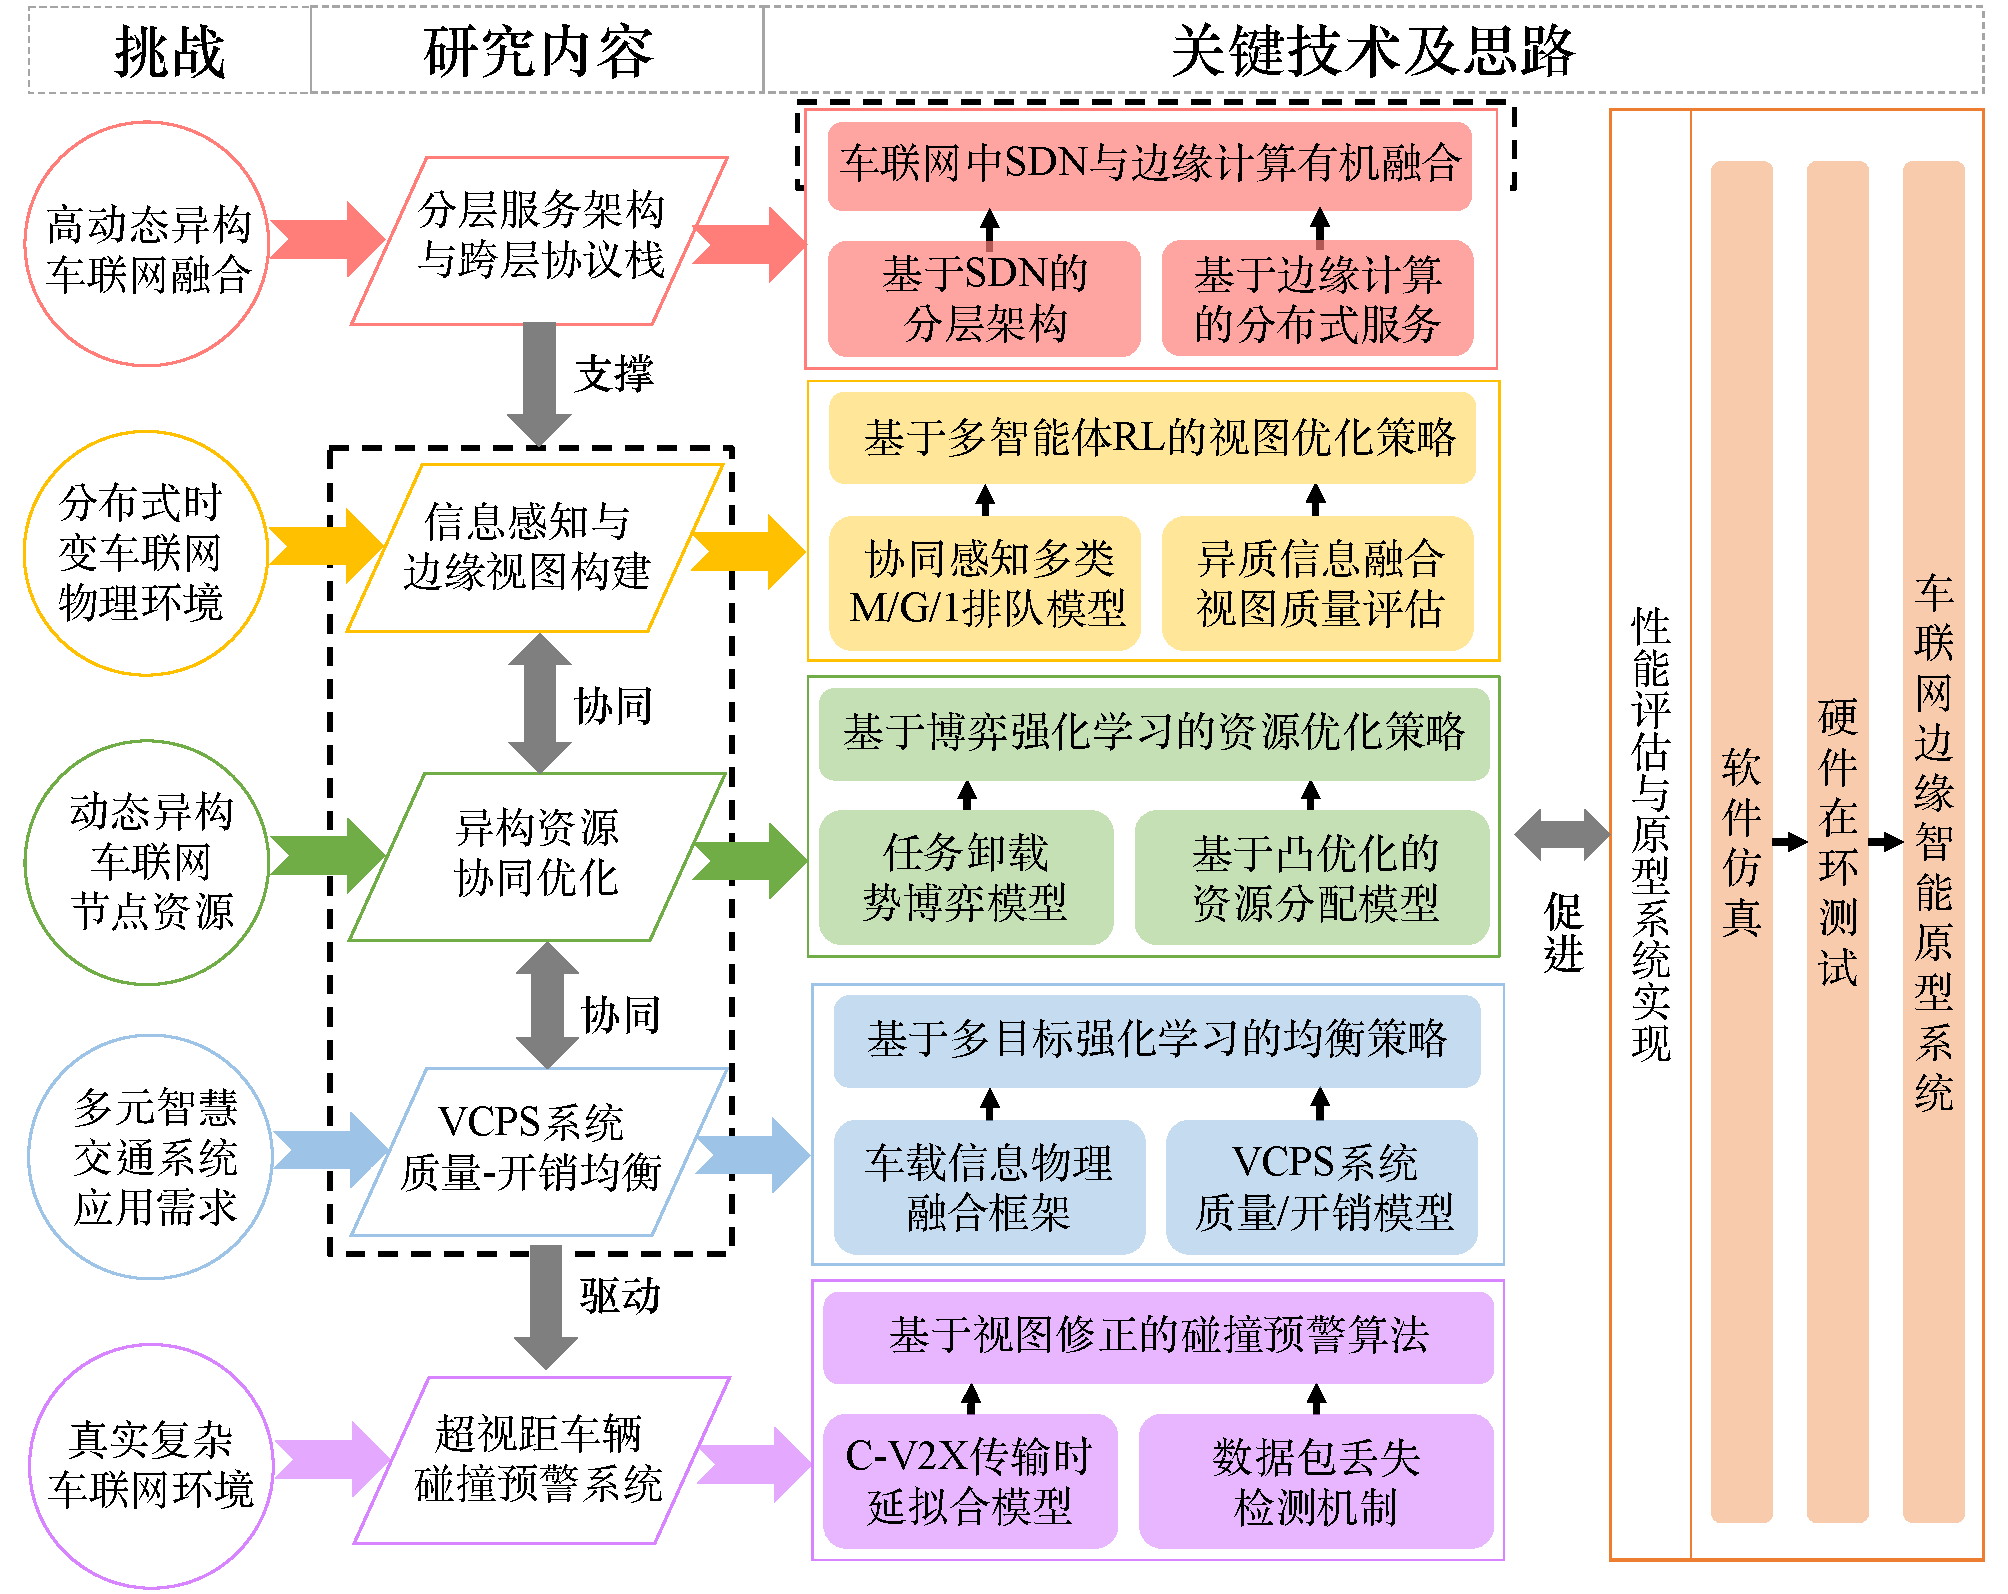
\includegraphics[width=1\columnwidth]{Fig1-5-technology-route.pdf}
	\bicaption{技术路线}{Technology route}
	\label{fig 1-5}
\end{figure}

本文技术路线如图 \ref{fig 1-5} 所示。首先,凝练关键科学问题:针对高动态异构车联网、分布式时变物理环境、动态异构节点资源、多元智能交通系统应用需求,以及真实复杂车联网环境所带来的挑战,从异构车联网融合、视图评估指标设计、异构资源协同优化、质量-开销均衡,以及原型系统设计与实现五方面协同驱动面向异构车联网的车载信息物理融合系统。
在此基础上,制定本文研究内容:1)研究面向异构车联网的分层服务架构和跨层协议栈,实现基于 SDN 的逻辑集中控制与基于边缘计算的分布式服务有机结合,为实现车载信息物理融合提供服务架构基础。2)研究车载边缘计算环境下协同信息感知与边缘视图构建,设计边缘视图评估指标,为实现车载信息物理融合系统提供数据支撑。3)研究 NOMA 车载边缘计算环境下异构资源协同优化策略,提高资源利用率,为实现车载信息物理融合提供技术支持。4)研究面向车载信息物理融合系统的质量-开销均衡优化策略,实现VCPS质量-开销均衡,为实现车载信息物理融合系统提供理论保障。5)研究基于车载信息物理融合的超视距碰撞预警系统原型,为实现车载信息物理融合系统提供系统验证。

最后,整理本文关键技术及思路:
1)首先,提出基于软件定义网络的集中控制分层框架;其次,提出基于车载边缘计算的分布式服务策略与跨层协议栈;最后,提出实现车联网中 SDN 与边缘计算有机融合的异构车联网服务架构。
2)首先,提出基于多类 M/G/1 优先队列的协同感知模型;其次,提出异质信息融合模型并设计边缘视图质量评估指标;最后,提出基于多智能体强化学习的视图优化策略,实现边缘视图构建。
3)首先,建立面向任务卸载的势博弈模型;其次,基于凸优化理论,提出通信资源分配模型;最后,基于博弈强化学习,将任务卸载博弈转变为利用基于多智能体 D4PG 算法进行求解,实现异构资源协同优化。
4)首先,建立车载信息物理融合框架;其次,提出 VCPS 质量模型与开销模型;最后,基于多目标强化学习,设计 VCPS 质量-开销均衡优化策略。
5)首先,提出基于C-V2X的无线传输时延拟合模型;其次,提出数据包丢失检测机制;最后,设计基于视图修正的碰撞预警算法,实现超视距碰撞预警系统原型。
6)搭建软件仿真环境、硬件在环测试平台,验证所提模型、机制与算法的可行性与有效性。在此基础上,针对具体应用场景,搭建系统原型,实现理论与应用相互促进。

\section{论文的特色与创新之处}\label{section 1-6}

本文致力于从服务架构、数据建模、资源调度、系统优化,以及原型实现五个层面协同研究并提炼面向异构车联网的车载信息物理融合关键科学问题,重点突破以下技术瓶颈:异构车联网融合、边缘视图评估与优化、异构资源协同优化、VCPS质量-开销均衡优化,以及原型系统设计与实现。
特别地,区别于现有单纯针对车联网的通信协议、服务架构、资源分配与智能应用等研究,本文从驱动面向异构车联网的车载信息物理融合系统的实际需求出发,分析当前面临的挑战,并针对车载信息物理融合系统的架构基础、数据支撑、技术支持、理论保障与原型系统五个方面提出关键问题。
本文具体特色体现在:
a)面对高异构、高动态、高分布式车联网环境,考虑车联网环境中的异构无线通信与移动数据节点所带来的挑战,研究如何将基于SDN的集中控制与基于边缘计算的分布式调度有机结合,为车载信息物理融合系统提供架构基础;
b)面向信息感知的时效性与准确性需求,考虑感知信息时变性、车辆节点移动性与感知能力差异性所带来的挑战,研究如何在车载边缘侧建立有效的逻辑视图,为车载信息物理融合系统提供数据支撑;
c)面向具有域内与域内干扰的 NOMA 车载边缘计算环境,考虑不同节点资源的动态异构性所带来的挑战,研究如何实现边缘协同最大化异构资源利用效率,为车载信息物理融合系统提供技术支持;
d)面向多元智能交通系统应用需求,考虑车联网中不同交通要素数字孪生质量/开销需求差异带来的挑战,研究如何实现车载信息物理融合系统质量-开销均衡,为车载信息物理融合系统提供理论保障;
e)面向真实复杂车联网环境,考虑基于真实 C-V2X 通信设备部署与实现原型系统所带来的挑战,研究基于车载信息物理融合的超视距碰撞预警系统原型设计与实现,为车载信息物理融合系统提供系统验证。
本文主要创新点概括如下。

\circled{1} 提出综合 SDN、NFV、边缘计算与网络切片关键思想的异构融合车联网服务架构:现有车联网服务架构相关研究主要关注于单一范式的实践应用,同时,大多研究也为给出其中具体实现细节与深度思考,难以适用于具有大规模数据服务需求的下一代车联网场景与支撑车载信息物理融合系统。基于此,本文首先综合考虑高移动数据节点、高动态网络拓扑、高异构通信资源、高分布式系统环境等车联网特征,设计基于 SDN 集中控制与基于边缘计算分布式服务有机结合的异构车联网架构,并提出跨层协议栈,实现异构车联网有机融合。

\circled{2} 定义边缘视图概念,率先设计视图评估指标并建立视图质量评估模型,提出分布式协同信息感知与异质信息融合的边缘视图构建机制:现有研究重点关注于针对单一类型的时态数据建模与调度,难以面向异构车联网的车载信息物理融合系统形成有效的数据支撑。基于此,本文首先综合考虑感知信息的时效性、完整性与一致性,定义车联网边缘视图概念,建立针对视图质量的量化评估模型,并提出基于多智能体强化学习的边缘视图优化策略,实现车载边缘计算环境下的有效信息物理融合。

\circled{3} 提出基于边缘协同的异构资源协同优化策略,打破传统针对单一资源的优化模式:现有面向车联网资源优化策略的研究主要集中于单一资源(通信、计算)的优化,难以满足不同任务对于车联网节点异构资源的需求。基于此,本文首先针对协同资源优化问题进行分解,将其转化为任务卸载与通信资源分配两个子问题。进一步,将任务卸载子问题建模为势博弈模型,并证明其具有纳什均衡与收敛性。最后,针对任务卸载博弈,提出基于多智能体 D4PG 算法的任务卸载策略,针对通信资源分配,提出基于凸优化的通信资源分配策略。

\circled{4} 定义车载信息物理融合系统质量与开销模型,提出基于多目标强化学习的优化策略,注重于实现 VCPS 质量最大化的同时,满足 VCPS 开销最小:现有研究主要关注于基于车载信息物理融合系统的应用,忽略了车载信息物理融合过程中构建质量与开销。基于此,本文首先面向多元智能交通系统应用的差异性需求,针对车联网中不同要素建立数字孪生模型。进一步,提出面向车联网中不同实体要素数字孪生的质量/开销模型。最后,基于多目标强化学习提出车载信息物理融合系统质量-开销均衡优化策略,实现VCPS质量-开销均衡。

\circled{5} 实现基于车载信息物理融合的超视距碰撞预警原型系统,在真实车联网环境下验证所提算法与系统模型:现有研究主要关注于基于仿真平台的实验验证,难以满足基于车载信息物理融合的实际 ITS 应用在真实车联网环境下的验证需求。基于此,本文首先建立基于C-V2X的无线传输时延拟合模型。进一步,提出数据包丢失检测机制。最后基于车载信息物理融合,设计基于视图修正的碰撞预警算法,实现超视距碰撞预警系统原型。

综上,本文建立在充分了解国内外相关领域学科前沿、清晰认识亟待解决的关键问题、合理制定研究目标与内容的基础上,是一项紧跟国际前沿的创新研究课题,是一项突破技术瓶颈的基础研究课题,也是一项理论结合实际的交叉研究课题。
本研究工作以车联网特征和智能交通系统应用需求为出发点,以车载信息物理融合为对象,以实现面向异构车联网的车载信息物理融合系统为目标,凝练出异构车联网融合、边缘视图评估与构建、异构资源协同优化、VCPS 质量-开销均衡,以及原型系统设计与实现五方面的关键问题,并针对服务架构融合、评估指标设计、资源协同优化、质量-开销均衡和原型系统实现进行深入研究,提出了面向异构车联网的车载信息物理融合新架构、新指标、新模型、新理论和新算法,致力于实现车载信息物理融合,以支持多元智能交通系统。
本文研究成果有助于完善车载信息物理融合理论体系,有助于推动智能交通系统及相关应用的标准制定与技术研发,是有研究特色、有理论意义、有实用价值的。

\section{论文的组织结构}\label{section 1-7}
本文围绕异构车联网中车载信息物理融合系统相关问题展开了研究。
具体地,本文将结合车联网特征、智能交通系统多元需求,从车联网的服务架构融合、评估指标设计、资源协同优化、质量-开销均衡,以及原型系统实现方面进行理论研究与技术创新。
本文共分为 7 章节,详细内容如下。

第一章,绪论。首先,介绍了车载信息物理融合系统的研究背景和国内外相关研究现状。其次,阐述了本文的研究目标与详细内容。最后,总结了本文的组织结构。

第二章,基于软件定义网络和边缘计算的异构车联网架构研究。首先,提出了基于软件定义网络的分层服务架构,并介绍了网络功能虚拟化和网络切片,以及基于边缘计算的车联网服务。其次,详细阐述了控制层、虚拟化层、数据层面临的挑战,并设计了跨层协议栈。最后,通过真实场景中的案例研究对应用层的无线传输时延进行了拟合与分析,并给出了相应的启示。

第三章,面向车载边缘计算的VCPS评估指标(Age of View)设计与优化策略研究。首先,提出了面向车载信息物理融合系统的协同信息感知与异质信息融合框架。在此基础上,考虑到多元信息的时效性、一致性与完整性,设计了VCPS评估指标(Age of View,AoV), 并形式化定义了在车载边缘计算环境下最大化AoV问题。然后,提出了基于多智能体强化学习的调度算法。最后,构建了实验仿真模型并验证了所提指标与算法的优越性。

第四章,面向NOMA车载边缘计算的异构资源协同优化策略研究。首先,提出了面向NOMA车联网的车载边缘计算架构。其次,建立了V2I传输模型和任务卸载模型,在此基础上,形式化定义了协同资源优化问题。再次,将原问题建模为具有纳什均衡的势博弈模型,并设计了基于多智能体D4PG的任务卸载算法和基于凸优化的资源分配算法。最后,建立了实验仿真模型并验证了所提算法的优越性。

第五章,面向车载信息物理融合的质量-开销优化策略研究。首先,提出了面向车载边缘计算的车载信息物理融合架构。其次,建立了协同感知模型和V2I上传模型,在此基础上,形式化定义了VCPS系统质量和系统开销,并给出了最大化系统质量与最小化系统开销的双目标问题。再次,提出了基于多目标强化学习的优化算法。最后,构建了实验仿真模型并验证了所提算法的优越性。

第六章,基于车载信息物理融合的超视距碰撞预警原型系统设计与实现。首先,建立了基于C-V2X的无线传输时延拟合模型。其次,提出了数据包丢失检测机制。最后,基于车载信息物理融合,设计了基于视图修正的车辆碰撞预警算法,实现超视距碰撞预警系统原型。

第七章,总结和展望。总结了全文研究的内容和贡献,并讨论了未来的研究方向与计划。






